%!TEX root = ../thesis.tex

\chapter{Grundlagen}

Im nachfolgenden werden Grundlagen erläutert, die als Basis des Projects dienen, so wie zum Verständnis des Kapitels `Frameworks' erforderlich sind.


\section{Cross Device Entwicklung}
Lorem ipsum dolor sit amet, consetetur sadipscing elitr, sed diam nonumy eirmod tempor invidunt ut labore et dolore magna aliquyam erat, sed diam voluptua. At vero eos et accusam et justo duo dolores et ea rebum. Stet clita kasd gubergren, no sea takimata sanctus est Lorem ipsum dolor sit amet. Lorem ipsum dolor sit amet, consetetur sadipscing elitr, sed diam nonumy eirmod tempor invidunt ut labore et dolore magna aliquyam erat, sed diam voluptua. At vero eos et accusam et justo duo dolores et ea rebum. Stet clita kasd gubergren, no sea takimata sanctus est Lorem ipsum dolor sit amet.

\section{Cross Platform Entwicklung}
Lorem ipsum dolor sit amet, consetetur sadipscing elitr, sed diam nonumy eirmod tempor invidunt ut labore et dolore magna aliquyam erat, sed diam voluptua. At vero eos et accusam et justo duo dolores et ea rebum. Stet clita kasd gubergren, no sea takimata sanctus est Lorem ipsum dolor sit amet. Lorem ipsum dolor sit amet, consetetur sadipscing elitr, sed diam nonumy eirmod tempor invidunt ut labore et dolore magna aliquyam erat, sed diam voluptua. At vero eos et accusam et justo duo dolores et ea rebum. Stet clita kasd gubergren, no sea takimata sanctus est Lorem ipsum dolor sit amet.

\section{Komponenten}

Lorem ipsum dolor sit amet, consetetur sadipscing elitr, sed diam nonumy eirmod tempor invidunt ut labore et dolore magna aliquyam erat, sed diam voluptua. At vero eos et accusam et justo duo dolores et ea rebum. Stet clita kasd gubergren, no sea takimata sanctus est Lorem ipsum dolor sit amet. Lorem ipsum dolor sit amet, consetetur sadipscing elitr, sed diam nonumy eirmod tempor invidunt ut labore et dolore magna aliquyam erat, sed diam voluptua. At vero eos et accusam et justo duo dolores et ea rebum. Stet clita kasd gubergren, no sea takimata sanctus est Lorem ipsum dolor sit amet.

\subsection{Kapsellung}
Lorem ipsum dolor sit amet, consetetur sadipscing elitr, sed diam nonumy eirmod tempor invidunt ut labore et dolore magna aliquyam erat, sed diam voluptua. At vero eos et accusam et justo duo dolores et ea rebum. Stet clita kasd gubergren, no sea takimata sanctus est Lorem ipsum dolor sit amet. Lorem ipsum dolor sit amet, consetetur sadipscing elitr, sed diam nonumy eirmod tempor invidunt ut labore et dolore magna aliquyam erat, sed diam voluptua. At vero eos et accusam et justo duo dolores et ea rebum. Stet clita kasd gubergren, no sea takimata sanctus est Lorem ipsum dolor sit amet.

\subsection{Web Components}
Lorem ipsum dolor sit amet, consetetur sadipscing elitr, sed diam nonumy eirmod
tempor invidunt ut labore et dolore magna aliquyam erat, sed diam voluptua. At vero eos et accusam et justo duo dolores et ea rebum. Stet clita kasd gubergren, no sea takimata sanctus est Lorem ipsum dolor sit amet. Lorem ipsum dolor sit amet, consetetur sadipscing elitr, sed diam nonumy eirmod tempor invidunt ut labore et dolore magna aliquyam erat, sed diam voluptua. At vero eos et accusam et justo duo dolores et ea rebum. Stet clita kasd gubergren, no sea takimata sanctus est Lorem ipsum dolor sit amet.

\subsubsection{Features}
Lorem ipsum dolor sit amet, consetetur sadipscing elitr, sed diam nonumy eirmod tempor invidunt ut labore et dolore magna aliquyam erat, sed diam voluptua. At vero eos et accusam et justo duo dolores et ea rebum. Stet clita kasd gubergren, no sea takimata sanctus est Lorem ipsum dolor sit amet. Lorem ipsum dolor sit amet, consetetur sadipscing elitr, sed diam nonumy eirmod tempor invidunt ut labore et dolore magna aliquyam erat, sed diam voluptua. At vero eos et accusam et justo duo dolores et ea rebum. Stet clita kasd gubergren, no sea takimata sanctus est Lorem ipsum dolor sit amet.

\subsubsection{Vorteile}
Lorem ipsum dolor sit amet, consetetur sadipscing elitr, sed diam nonumy eirmod tempor invidunt ut labore et dolore magna aliquyam erat, sed diam voluptua. At vero eos et accusam et justo duo dolores et ea rebum. Stet clita kasd gubergren, no sea takimata sanctus est Lorem ipsum dolor sit amet. Lorem ipsum dolor sit amet, consetetur sadipscing elitr, sed diam nonumy eirmod tempor invidunt ut labore et dolore magna aliquyam erat, sed diam voluptua. At vero eos et accusam et justo duo dolores et ea rebum. Stet clita kasd gubergren, no sea takimata sanctus est Lorem ipsum dolor sit amet.

\subsubsection{Polyfills}
Lorem ipsum dolor sit amet, consetetur sadipscing elitr, sed diam nonumy eirmod tempor invidunt ut labore et dolore magna aliquyam erat, sed diam voluptua. At vero eos et accusam et justo duo dolores et ea rebum. Stet clita kasd gubergren, no sea takimata sanctus est Lorem ipsum dolor sit amet. Lorem ipsum dolor sit amet, consetetur sadipscing elitr, sed diam nonumy eirmod tempor invidunt ut labore et dolore magna aliquyam erat, sed diam voluptua. At vero eos et accusam et justo duo dolores et ea rebum. Stet clita kasd gubergren, no sea takimata sanctus est Lorem ipsum dolor sit amet.

\section{Typescript}

\subsection{Entwicklung von Javascript}

Javascript wurde erstmals 1996 von Brendan Eich in einer Implementierung des Netscape Navigator Browsers eingeführt,
worauf weitere Browser die Syntax und APIs ähnlich, jedoch nicht identisch nach implementierten.
Daraufhin veröffentlichte die ECMA International einen Standard, welcher die Spezifikationen der neuen Sprache definieren sollte.
Dieser Standard trägt den namen ECMAScript und ist der offizielle und somit auch bekannteste Standard der Sprache.
ActionScript von Macromedia und JScript von Microsoft sind Implementierungen der Browsersprache,
die nicht dem ECMA Standard entsprechen, jedoch darauf aufbauen.

1997 wurde die erste Versionen des nun standardisiertem ECMAScript veröffentlicht. Ein Jahr später erschien bereits ECMAScript2,
allerdings beinhaltete dieses Update nur kleine Änderungen um einem parallel entstandenen ISO Standard von JavaScript zu implementieren.
Die nächste große Neuerung kam 1999 mit ECMAScript3, in welcher einige der bahnbrechenden Features implementiert wurden, die auch heute noch Kern von JavaScript sind
``..regular expressions, try/catch exception handling..''\cite{js-vs-es}.

ECMAScript4 sollte 2003 ein bahnbrechendes Upgrade für die Skriptsprache werden. Vom Standard wurden allerdings nur wenige Features implementiert.
Zur selben Zeit wurde jQuery gebohren um


2009 erschien ECMAScript5, mit vollem Support in allen verbreiteten Webbrowsern, abgesehen vom Internet Explorer.
Neue Features waren unter anderem JSON support und Array Funktionen wie map und forEach
Durch das blockieren einiger Features wurde JavaScript sauberer und stabiler.

ECMAScript6 sollte bereits 2013 veröffentlicht werden, der offizielle Releasetermin wurde dann allerdings bis in den Juni 2015 verschoben und ist bis heute noch nicht ausreichend in allen Browsern implementiert.
\cite{js-vs-es}


\begin{figure}[htbp]
 \centering
 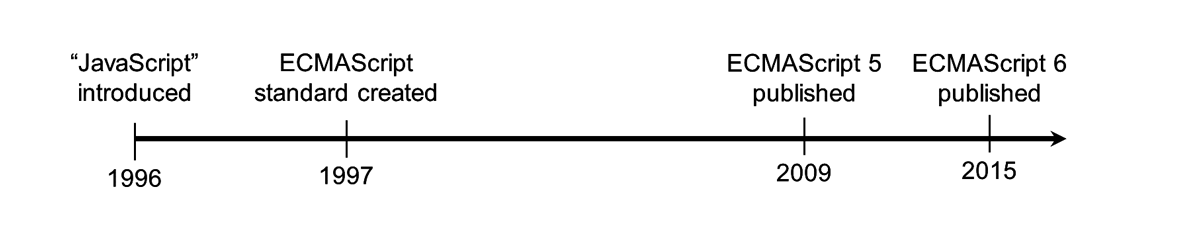
\includegraphics[width=\linewidth]{kapitel2/javascript-timeline.png}
 \caption{History of Javascript}\cite[28]{EssentialTS}
\end{figure}

\subsection{Transpilierung}
